\subsection{Interpreting Utilization}
\label{subsec:utilization}

Utilization can be characterized in many ways, and each definition can answer
a particular question. Furthermore, as stated in the previous section, multiple
parties may interpret utilization differently, based on their aims and requirements.


Utilization as the average data rate for each device in each time slot 
portrays the overall spacio-temporal aspect of our dataset. We plot a distribution
of the rate per device-time in figure~\ref{fig:CDF-data-rate-all}. This shows that
median utilization of household users is the same in both sets (50 kbps). A comparison
between the \test and \control set shows that there is no affect on the overall adoption.

\begin{figure}[ht!]
\centering
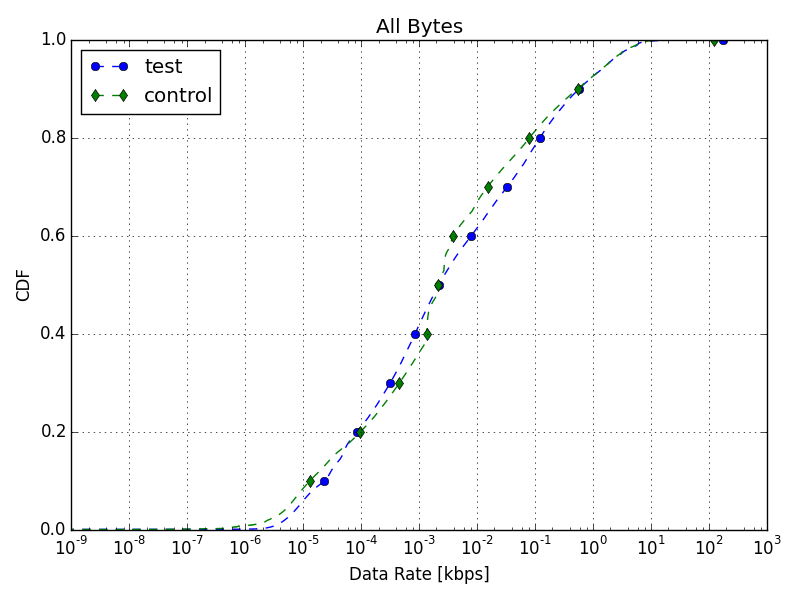
\includegraphics[width=0.90\linewidth]{figures/cdf-all-bytes.png}
  \caption{CDF of data rate per time slot for all devices (agg view of data): Overall not much change due to capacity increase. Median data rate ~ 2bps for 3 months x thousands of devices!}
  %http://sites.noise.gatech.edu/~sarthak/files/comcast/plots/full_dw/cdf-all-bytes.png
  \label{fig:CDF-data-rate-all}
\end{figure}

Based on the measurement methodology, we study the highest utilization seen by a household
both in its lifetime, and on each day. Our aim is to examine the peak usage per household, and
study if the behavior changes due to an upgrade.

Figure~\ref{fig:CDF-data-rate-max} provides a distribution of the highest average
data rate a household achieves. To avoid outliers, we also plot the 90\%-ile of the max
data rate achieved by households in both \test and \control sets. We see that a median
household is expected to achieve the highest data rate of between 1 -- 10 Mbps over its
lifetime. This is much lower than the access link capacity,
indicating that the median device has a utilization ratio (avg data rate:capacity) under
0.1 in our dataset. The number of households that increased their peak utilization beyond
the \control set's 105 Mbps capacity were negligible.

Surprisingly, we see that 30\% of the households from the \test set have a low peak
utilization (under 0.1 Mbps), while 40\% of the \control set households are under 0.1 Mbps.
Thus, the absolute peak utilization does not increase when compared to the access link
capacity, but there is certainly an increase in peak utilization of devices that had a low
requirement, due to the change in capacity.

To investigate this further, we also study the \emph{peak utilization per device on a daily basis}.
Figure~\ref{fig:CDF-data-rate-max-daily} shows that for 30\% of the devices,
the maximum data rate in the \test set is consistently higher than the \control set, albeit
no where near the actual access link capacity.

This is similar to the behavior observed in figure~\ref{fig:TS-data-rate-daily}, showing that the peak
usage during prime-time is unaffected, but lower utilization throughout the day is higher
for the test set. We speculate that there could be two possible reasons for this increase
in utilization: (1) short term downloads and/or web browsing achieves a slightly better
data rate on a small time scale, or (2) real-time video quality is slightly higher, but
not enough to completely saturate the access link capacity. Unfortunately, we miss these
short lived, or consistent, events due to a 15 minute time slot granularity and only
looking at byte counters.


\paragraph{Different Perspectives of Utilization: }We take this opportunity to reflect on the
interpretation of the disparity of peak utilization per device, as shown in
figure~\ref{fig:CDF-data-rate-max}. The ISP may interpret this as no change in peak usage, as
the prime-time usage remained the same based on aggregated usage, even in prime-time. Thus, we
believe that given the opportunity, the provider will not invest to offer a higher access
link unless it in a region showing such low demand unless it is guaranteed profit, or is forced
into deployment by an external agency.

In contrast, the consumer (and therefore the FCC) might be convinced that individually
the usage behavior of a household is affected by the increase in access link
capacity, especially for households with a lower utilization. We believe that this is
the perspective the FCC takes when considering deployment and adoption of broadband services.

\begin{figure}[ht!]
%\hspace*{-0.2in}
\begin{minipage}{0.90\linewidth}
\centering
%
%\hfill
\begin{subfigure}[b]{0.90\linewidth}
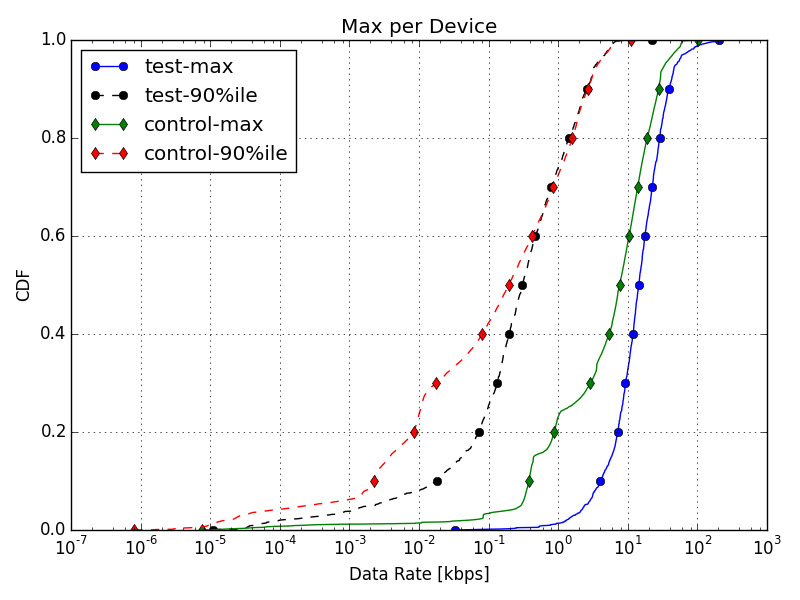
\includegraphics[width=\linewidth]{figures/cdf-max-per-device.png}
  \caption{CDF of max per device: test set has higher (max) average data rate below 10 kbps.  30\% of devices in the control set have a max data rate of 2 kbps while 30\% of test set has a max data rate of 10 kbps. (sanity check numbers, redo plot)}
  %http://sites.noise.gatech.edu/~sarthak/files/comcast/plots/full_dw/cdf-max-per-device.png
  \label{fig:CDF-data-rate-max}
\end{subfigure}
%
\vspace{-1em}
%
\begin{subfigure}[b]{0.90\linewidth}
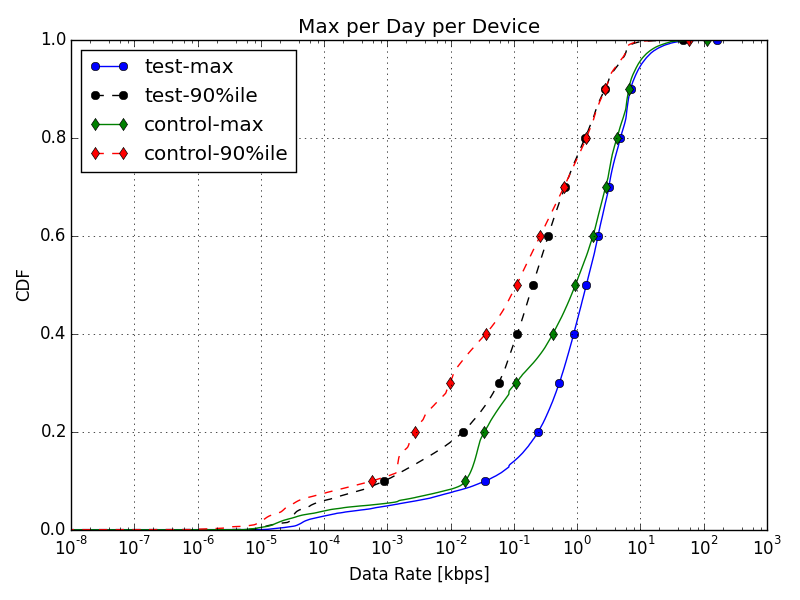
\includegraphics[width=\linewidth]{figures/cdf-max-per-day-per-device.png}
  \caption{CDF of max per device daily}
  \vspace{1em}
  %http://sites.noise.gatech.edu/~sarthak/files/comcast/plots/full_dw/cdf-max-per-day-per-device.png
  \label{fig:CDF-data-rate-max-daily}
\end{subfigure}
%\hfill
\end{minipage}
\caption{Peak Utilization: The maximum data rate varies for test and control set for low data rates, and this variation is present daily.}
\label{fig:peak-utilization}
% created using docs/metadata-separated.log
\end{figure}

% conclusion
\todo{needs work on conclusion}
Although our unbiased experiment still
shows a certain correlation between utilization and capacity, it also contradicts the
law of diminishing returns ~\cite{bischof2014broadband-behavior}. \todo{sanity check}